

%&from template
\documentclass[12pt]{article}\usepackage[]{graphicx}\usepackage[]{color}
%% maxwidth is the original width if it is less than linewidth
%% otherwise use linewidth (to make sure the graphics do not exceed the margin)
\makeatletter
\def\maxwidth{ %
  \ifdim\Gin@nat@width>\linewidth
    \linewidth
  \else
    \Gin@nat@width
  \fi
}
\makeatother

\definecolor{fgcolor}{rgb}{0.345, 0.345, 0.345}
\newcommand{\hlnum}[1]{\textcolor[rgb]{0.686,0.059,0.569}{#1}}%
\newcommand{\hlstr}[1]{\textcolor[rgb]{0.192,0.494,0.8}{#1}}%
\newcommand{\hlcom}[1]{\textcolor[rgb]{0.678,0.584,0.686}{\textit{#1}}}%
\newcommand{\hlopt}[1]{\textcolor[rgb]{0,0,0}{#1}}%
\newcommand{\hlstd}[1]{\textcolor[rgb]{0.345,0.345,0.345}{#1}}%
\newcommand{\hlkwa}[1]{\textcolor[rgb]{0.161,0.373,0.58}{\textbf{#1}}}%
\newcommand{\hlkwb}[1]{\textcolor[rgb]{0.69,0.353,0.396}{#1}}%
\newcommand{\hlkwc}[1]{\textcolor[rgb]{0.333,0.667,0.333}{#1}}%
\newcommand{\hlkwd}[1]{\textcolor[rgb]{0.737,0.353,0.396}{\textbf{#1}}}%
\let\hlipl\hlkwb

\usepackage{framed}
\makeatletter
\newenvironment{kframe}{%
 \def\at@end@of@kframe{}%
 \ifinner\ifhmode%
  \def\at@end@of@kframe{\end{minipage}}%
  \begin{minipage}{\columnwidth}%
 \fi\fi%
 \def\FrameCommand##1{\hskip\@totalleftmargin \hskip-\fboxsep
 \colorbox{shadecolor}{##1}\hskip-\fboxsep
     % There is no \\@totalrightmargin, so:
     \hskip-\linewidth \hskip-\@totalleftmargin \hskip\columnwidth}%
 \MakeFramed {\advance\hsize-\width
   \@totalleftmargin\z@ \linewidth\hsize
   \@setminipage}}%
 {\par\unskip\endMakeFramed%
 \at@end@of@kframe}
\makeatother

\definecolor{shadecolor}{rgb}{.97, .97, .97}
\definecolor{messagecolor}{rgb}{0, 0, 0}
\definecolor{warningcolor}{rgb}{1, 0, 1}
\definecolor{errorcolor}{rgb}{1, 0, 0}
\newenvironment{knitrout}{}{} % an empty environment to be redefined in TeX

\usepackage{alltt}
\usepackage{amsmath}
\usepackage{graphicx}
\usepackage{enumerate}
\usepackage{natbib}
\usepackage{url} % not crucial - just used below for the URL
% \usepackage[strings]{underscore}

%% added by author (CJ)
\usepackage{tikz}
\usepackage{floatpag}\floatpagestyle{empty}

\usetikzlibrary{calc,fit,positioning,arrows,shapes,backgrounds}
\tikzset{>={latex}}
\definecolor{dagblue}{rgb}{0.81,0.902,0.957}
\usepackage{bm}
\graphicspath{{/home/chris/uncertainty/evi/hiv/},{c:/Users/chris/Dropbox/work/uncertainty/evi/hiv/}}

\DeclareMathOperator*{\argmin}{arg\,min} 
\DeclareMathOperator*{\argmax}{arg\,max} 

%\pdfminorversion=4
% NOTE: To produce blinded version, replace "0" with "1" below.
\newcommand{\blind}{1}

% DON'T change margins - should be 1 inch all around.
\addtolength{\oddsidemargin}{-.5in}%
\addtolength{\evensidemargin}{-.5in}%
\addtolength{\textwidth}{1in}%
\addtolength{\textheight}{-.3in}%
\addtolength{\topmargin}{-.8in}%

\newcommand{\cov}{\mbox{cov}}
\newcommand{\var}{\mbox{var}}
\newcommand{\logit}{\mbox{logit}}
%\newcommand{\det}{\mbox{det}}
\newcommand{\y}{\mathbf{y}}
\newcommand{\x}{\mathbf{x}}
%\newcommand{\max}{\mathbf{max}}
%\newcommand{\min}{\mathbf{min}}
\newcommand{\cc}{\mathbf{c}}
\newcommand{\pinodelta}{\overline{(\pi\delta)}}
\newcommand{\pidelta}{(\pi\delta)}
\IfFileExists{upquote.sty}{\usepackage{upquote}}{}
\IfFileExists{upquote.sty}{\usepackage{upquote}}{}
\IfFileExists{upquote.sty}{\usepackage{upquote}}{}
\begin{document}

%\bibliographystyle{natbib}

\def\spacingset#1{\renewcommand{\baselinestretch}%
{#1}\small\normalsize} \spacingset{1}


%%%%%%%%%%%%%%%%%%%%%%%%%%%%%%%%%%%%%%%%%%%%%%%%%%%%%%%%%%%%%%%%%%%%%%%%%%%%%%

\if0\blind
{
  \title{\bf Value of Information: Sensitivity Analysis and Research Design in Bayesian Evidence Synthesis\\~\\
  Supplementary figures}
  \author{Christopher Jackson, Stefano Conti, Anne Presanis, Daniela De Angelis
    \\
    MRC Biostatistics Unit, University of Cambridge\\
  }
  \maketitle
} \fi

\if1\blind
{
  \bigskip
  \bigskip
  \bigskip
  \begin{center}
    {\LARGE\bf Value of Information: sensitivity analysis and research design in Bayesian evidence synthesis\\~\\
  Supplementary figures}
\end{center}
  \medskip
} \fi

\bigskip

%%% TODO 





%% \begin{figure}
%% <<prevnums-base,dev='my_pdf', fig.ext='pdf'>>=
%% prev.plot(sam)
%% nums.plot(sam)
%% @
%%   \caption{Posterior distributions of HIV prevalence (top) and numbers of MSM living with HIV/AIDS (bottom), London 2012. Darkness within each strip proportional to posterior density, with 95\% credible intervals indicated.  Base case analysis in paper. }
%%   \label{fig:res:prev}
%% \end{figure}


\begin{figure}
\begin{knitrout}
\definecolor{shadecolor}{rgb}{0.969, 0.969, 0.969}\color{fgcolor}
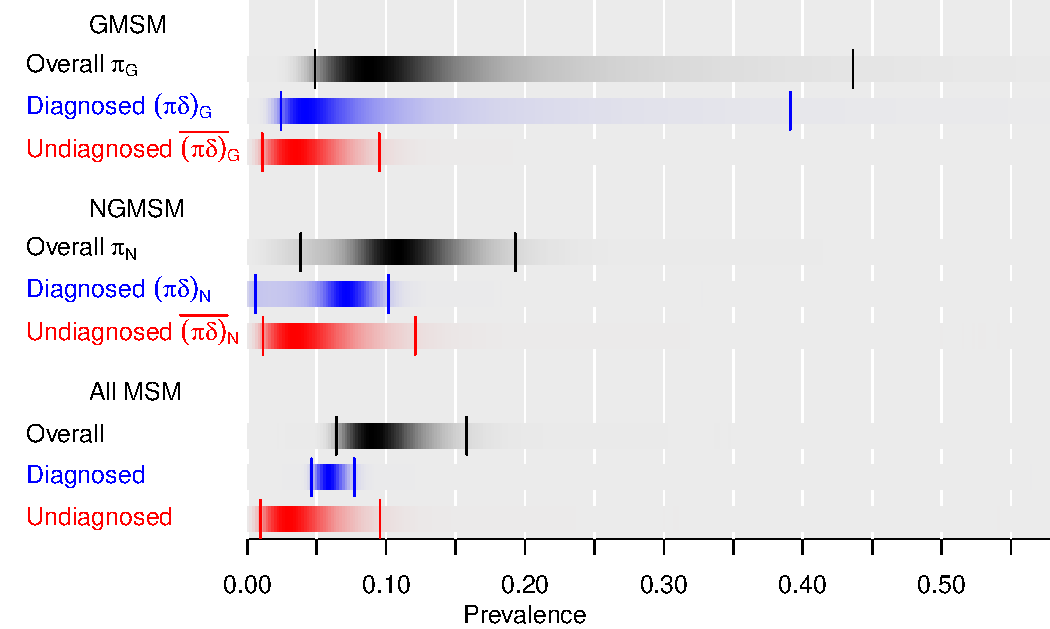
\includegraphics[width=\maxwidth]{figure/prevnums-nogu-1} 

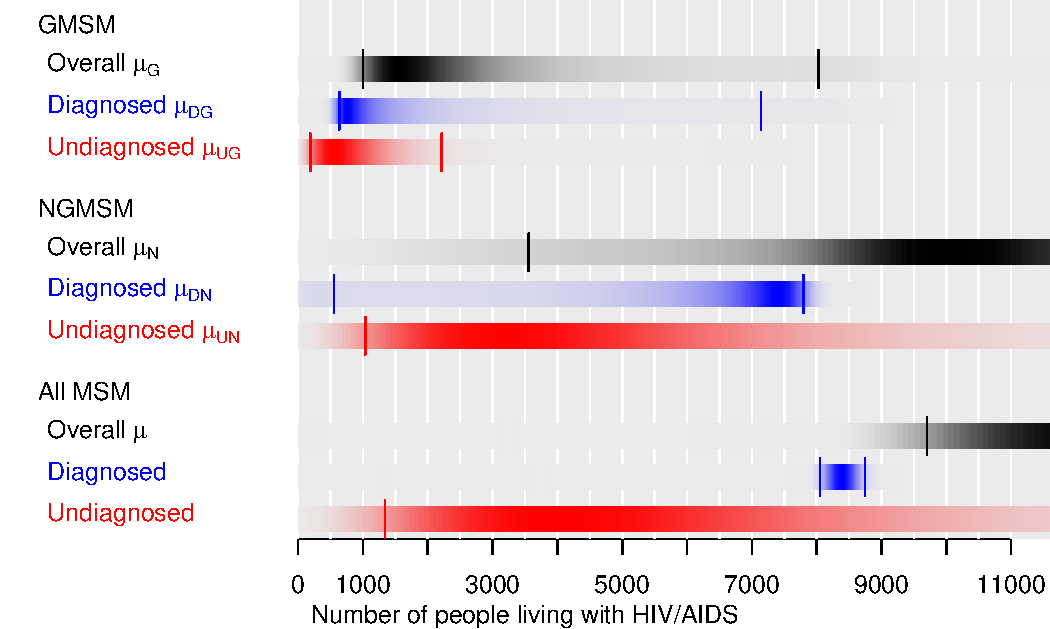
\includegraphics[width=\maxwidth]{figure/prevnums-nogu-2} 

\end{knitrout}
  \caption{Posterior distributions of HIV prevalence (top) and numbers of MSM living with HIV/AIDS (bottom), London 2012. Darkness within each strip proportional to posterior density, with 95\% credible intervals indicated. Alternative assumption (a): undiagnosed prevalence from GUM Anon only }
  \label{fig:res:prev}
\end{figure}


\begin{figure}
\begin{knitrout}
\definecolor{shadecolor}{rgb}{0.969, 0.969, 0.969}\color{fgcolor}
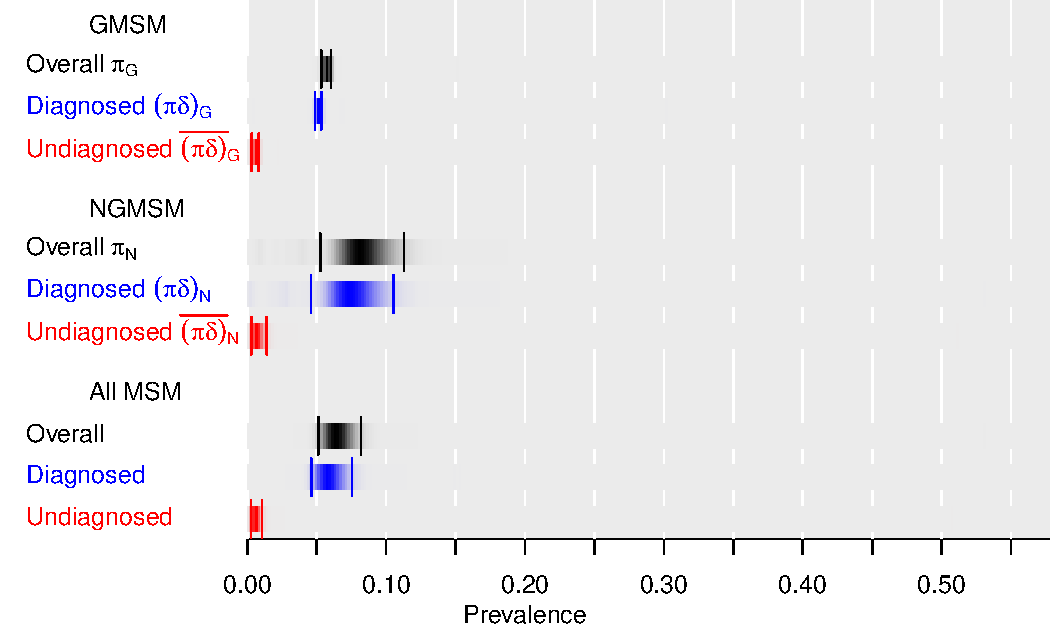
\includegraphics[width=\maxwidth]{figure/prevnums-gudnd-1} 

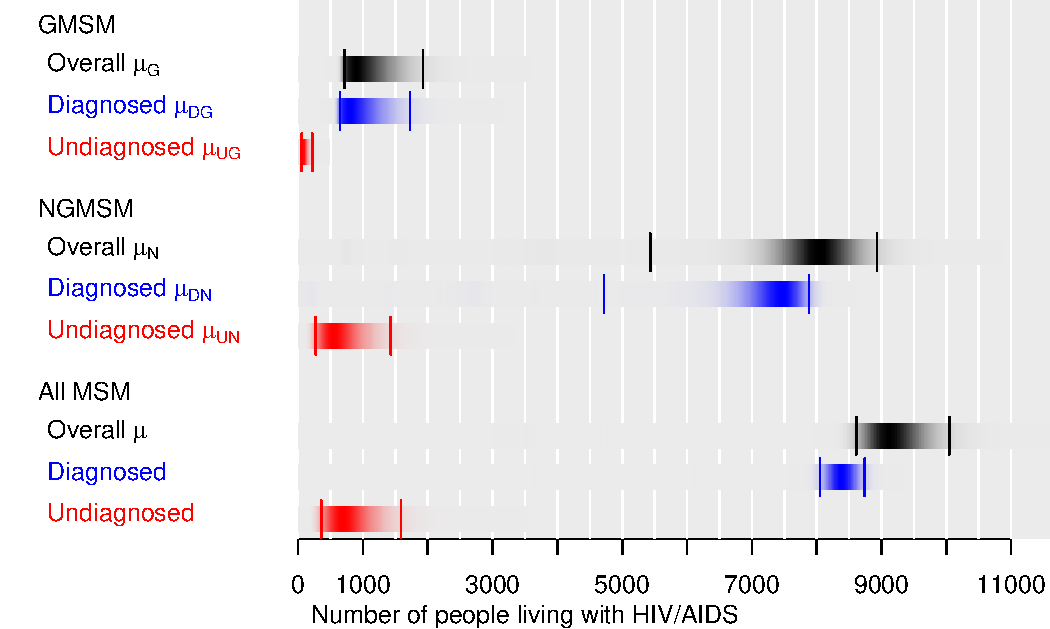
\includegraphics[width=\maxwidth]{figure/prevnums-gudnd-2} 

\end{knitrout}
  \caption{Posterior distributions of HIV prevalence (top) and numbers of MSM living with HIV/AIDS (bottom), London 2012. Darkness within each strip proportional to posterior density, with 95\% credible intervals indicated. Alternative assumption (b): GUMCAD also informs diagnosed prevalence }
  \label{fig:res:prev}
\end{figure}




%% \begin{figure}
%% <<evppi-base>>=
%%   evppi.plot(pe, phi, phimat)
%% @ 
%%   \caption{Expected value of partial perfect information in the HIV prevalence model.  Base case analysis in paper. }
%%   \label{fig:res:evppi}
%% \end{figure}


\begin{figure}
\begin{knitrout}
\definecolor{shadecolor}{rgb}{0.969, 0.969, 0.969}\color{fgcolor}
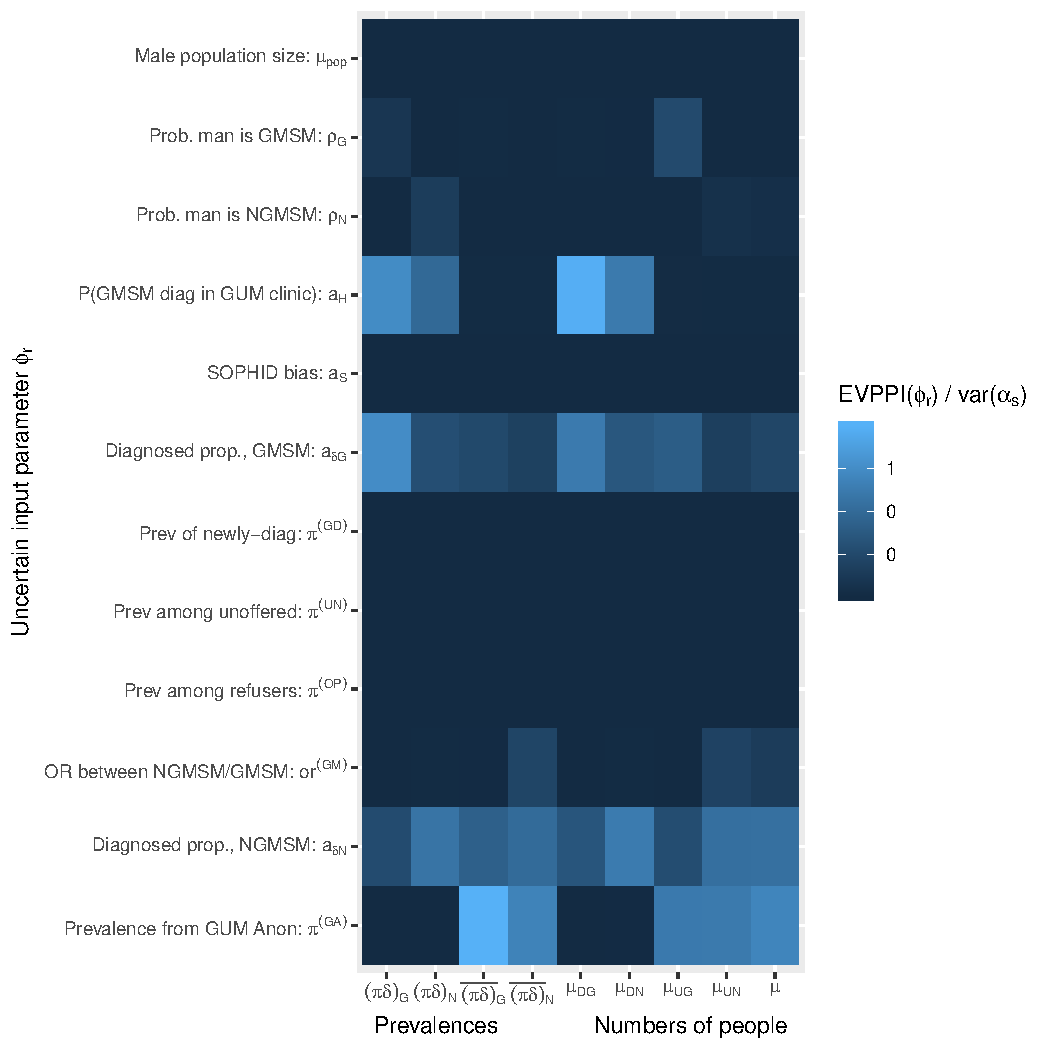
\includegraphics[width=\maxwidth]{figure/evppi-nogu-1} 

\end{knitrout}
  \caption{Expected value of partial perfect information in the HIV prevalence model.  Alternative assumption (a): undiagnosed prevalence from GUM Anon only }
  \label{fig:res:evppi}
\end{figure}


\begin{figure}
\begin{knitrout}
\definecolor{shadecolor}{rgb}{0.969, 0.969, 0.969}\color{fgcolor}
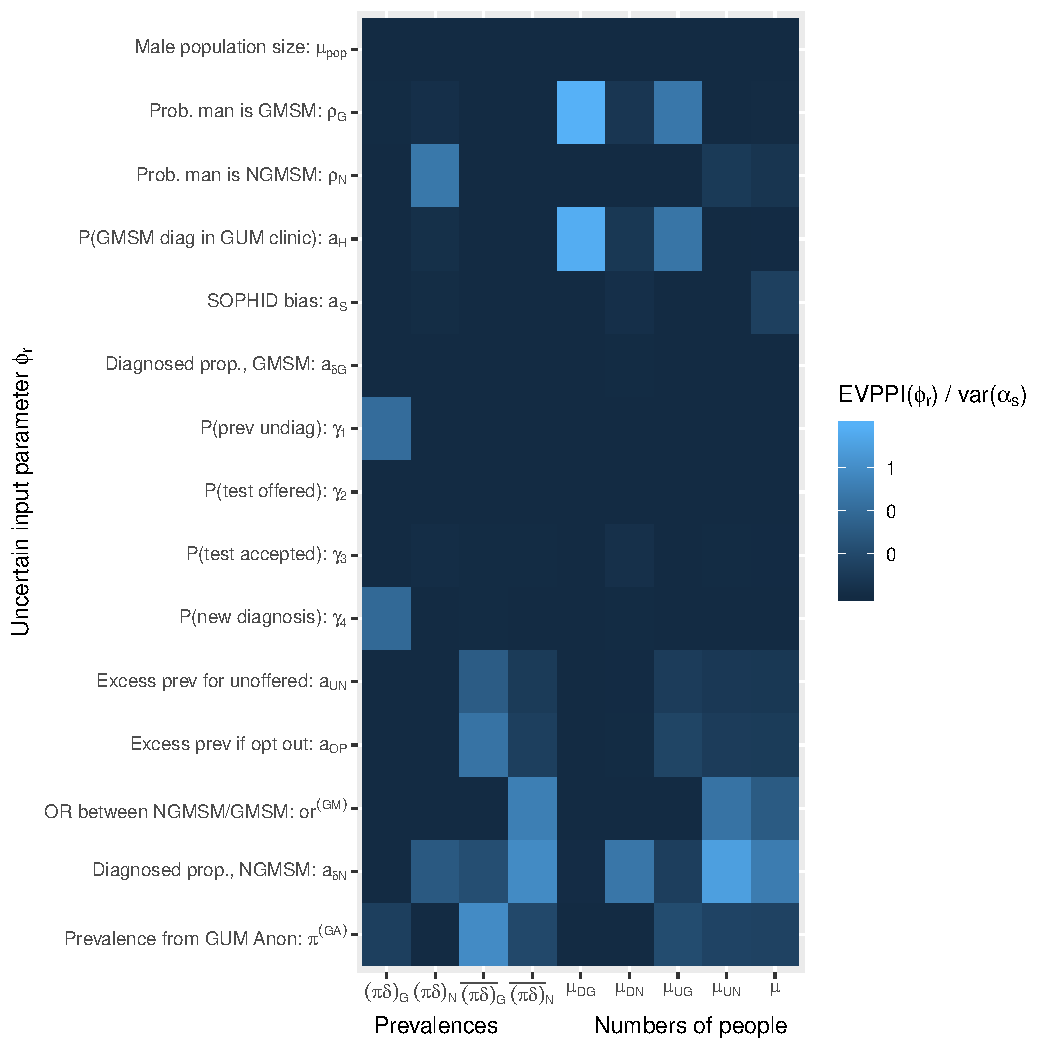
\includegraphics[width=\maxwidth]{figure/evppi-gudnd-1} 

\end{knitrout}
  \caption{Expected value of partial perfect information in the HIV prevalence model.  Alternative assumption (b): GUMCAD also informs diagnosed prevalence }
  \label{fig:res:evppi}
\end{figure}


\end{document}
